
We need to specify the gravity acceleration vector $\vec{g}$
inside the domain. 
We have several option. 

\begin{itemize}
\item the simplest option is to set $\vec{g} = - g_0 \vec{e}_r$
with $g_0$ being a constant (e.g. 9.8~\si{\meter\per\second}).
This is {\python gravity\_model=0}


\item We can assume the domain to be spherically symmetric: 
the core has a density $\rho_c$ and the mantle has a density $\rho_m$.
In that case we have
In the end we have:
\begin{eqnarray}
g_c(r)&=& \frac{1}{3}\hat{\rho}_c r \nn\\ 
g_m(r)&=& \frac{1}{3}\hat{\rho}_m r +\frac{C}{r^2} 
\end{eqnarray}
with 
\[
C=\frac{R_1^3}{3} (\hat{\rho}_c-\hat{\rho}_m)
\]
In the core we have $\vec{g}_c = - g_c(r) \vec{e}_r$
and in the mantle  $\vec{g}_m = - g_m(r) \vec{e}_r$.

\begin{center}
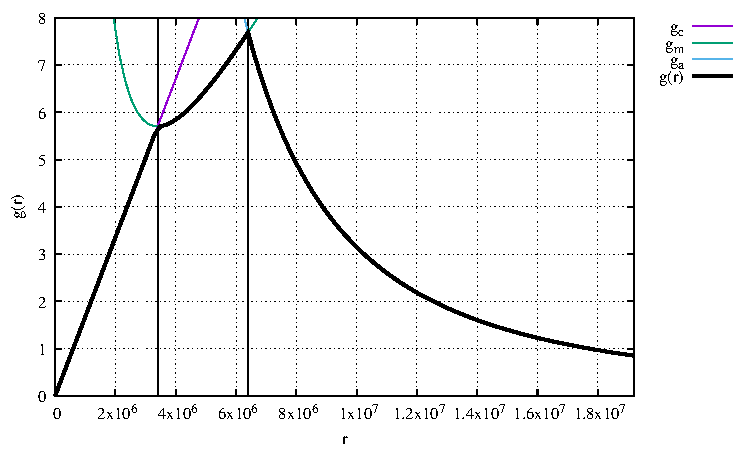
\includegraphics[width=8cm]{images/bench/g}
\end{center}

This is {\python gravity\_model=1}

\item This is no more an axisymmetric case. We have the same 
structure (core and mantle) but there is now a sphere ('blob')
of density $\rho_{blob}$ at location $x=0$ $z=z_{blob}$ of 
radius $R_{blob}$. 

The gravity field is then the sum of the spherically symmetric one 
above and the one generated by the density anomaly in the blob.

This is {\python gravity\_model=2}

\end{itemize}

